\subsection{Registered three-arm campaign: not admitted}
The complete four-job A/B/C2 gate fails because C2's F03 handoff fails. Consequently, \textbf{none of the planned 166 three-arm cells is executed}. The original grid and protocols remain unchanged. The three jobs that C2 passes are not substituted for the registered set, and its lack of a runtime model stage earns no financial discount. This is an economic admission failure grounded in delivered scope, not a requirement for actual sales.

\subsection{Separate accepted A/B diagnostic}
A new, explicitly exploratory diagnostic was registered after production and before its economic outcomes. It includes all four accepted A/B jobs, the same exact B asset and all 24 already prospective no-benefit stress cases with eight paired seeds. The original three-arm adapter is not weakened. A separate acceptance schema verifies every A/B job and independent audit row; C2 has no financial curve in this diagnostic.

Its prediction was stated before execution. When A and B have equal assumed complete nominal operating cost and no measured value, effort or capacity premium, incremental saving is zero. Positive construction cost, upkeep or interruption cannot create a positive repayment case. The model should refuse construction even if the underlying service occasionally earns a surplus. This prediction is algebraic; the executions test whether competition, cash timing, rejection and accounting respect it. They are not a new empirical estimate that B's true savings equal zero.

The campaign completes 192 paired worlds and 384 enterprise histories. A separate Python arithmetic audit reconciles every history without failure. It reconstructs 8,021 B decision-time earned-cash values and verifies that each investment consideration identifies the exact tested B asset. Every registered decision also lacks sufficient earned cash under the inherited reserve rule: the highest decision-time earned amount available is minus \$108. Thus both nonpositive incremental repayment and funding constraints bind in these histories; the observed refusals should not be attributed to only one of them. There are \textbf{zero constructions, zero earned-funded constructions and zero incremental B profit in every paired world}. Every operational A/B summary matches. The 2,066 delivery attempts are 1,033 per arm in paired copies, not independent real customers.

Twelve of 192 worlds per arm earn a positive modeled operating profit. Across all individual worlds, profit ranges from a loss of \$310 to a gain of \$86; every scenario's mean profit is negative. Positive service profit therefore does not justify the new asset. Its full bill is never charged as a completed modeled construction because no investment proceeds; the actual research construction that produced it occurred outside the simulation and remains explicitly unpriced in the historical account. Those modeled receipts did not finance this research.

\begin{table}[htbp]
\centering\small
\begin{tabularx}{\textwidth}{Xrrrr}
\toprule
Stress & \multicolumn{2}{c}{Mean profit (USD)} & \multicolumn{2}{c}{Mean accepted}\\
 & Determ. & Logit & Determ. & Logit\\
\midrule
Reference & -154.00 & -40.25 & 0.000 & 7.875\\
Zero demand & -154.00 & -154.00 & 0.000 & 0.000\\
Low demand & -154.00 & -107.12 & 0.000 & 3.125\\
Target \$10 & -116.19 & -96.81 & 10.750 & 13.500\\
Target \$5; floor \$6 & -149.50 & -144.38 & 22.875 & 20.625\\
Stronger, cheaper AI & -154.00 & -146.50 & 0.000 & 0.500\\
Cheaper human provider & -154.00 & -66.50 & 0.000 & 6.000\\
Competitor price response & -104.94 & -11.19 & 3.500 & 10.125\\
Delayed collections & -154.00 & -50.25 & 0.000 & 7.875\\
Quality failures & -145.88 & -93.06 & 1.250 & 5.000\\
Maintenance shock & -154.00 & -40.25 & 0.000 & 7.875\\
Cash and capacity stress & -310.00 & -306.88 & 0.000 & 0.625\\
\bottomrule
\end{tabularx}
\caption{All twelve diagnostic stresses, eight seeds per buyer rule. A and B have identical outcomes, zero investments and unknown actual monetary cost. Simulated accepted counts are not observed customer jobs.}
\end{table}


\begin{figure}[htbp]
\centering
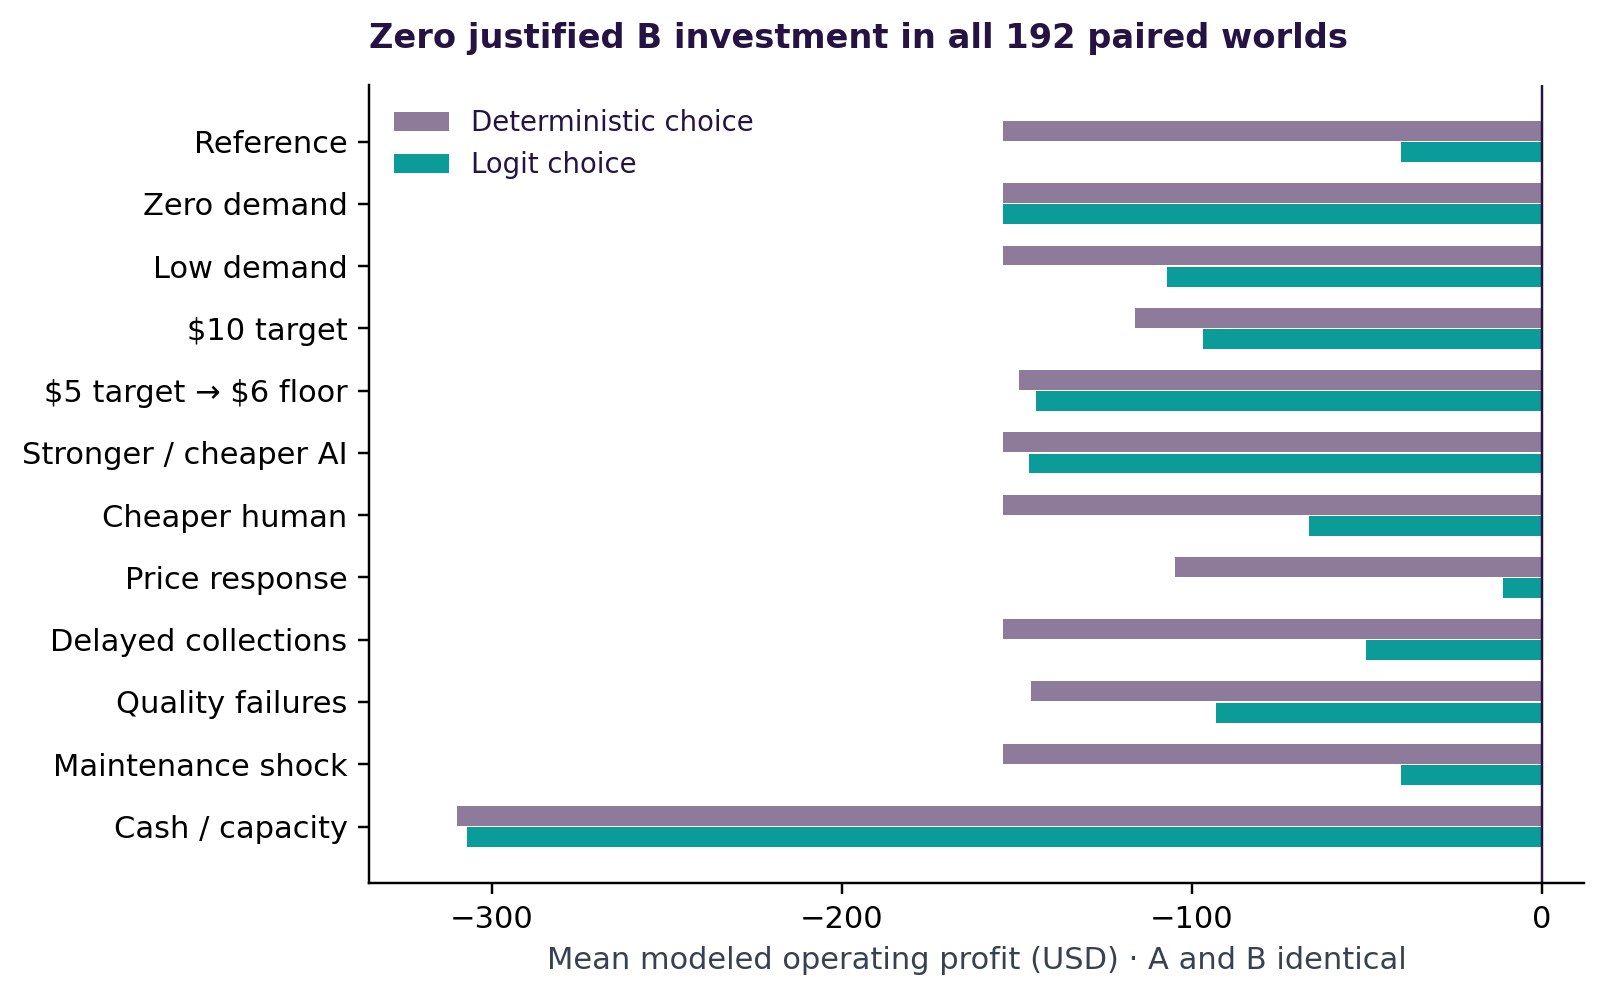
\includegraphics[width=\textwidth]{market-diagnostic.png}
\caption{Mean operating profit under both buyer-choice rules for every registered A/B diagnostic stress. A and B coincide in all paired worlds. These conditional outputs are not demand estimates; no scenario mean is profitable and no B investment proceeds.}
\end{figure}

The reference deterministic rule buys no enterprise output and incurs \$154 in setup and weekly overhead. The reference logit rule averages 7.875 accepted deliveries and a \$40.25 loss, with two profitable worlds. Alternative buyer modeling therefore changes allocation and service viability without producing a capability-investment case. A \$10 target produces more accepted work but insufficient mean margin. The \$5 target is actually floored at \$6 by the retained nominal-cost-plus-\$1 policy; its higher volume still does not recover overhead on average.

Stronger low-cost AI sharply reduces the logit enterprise's accepted volume. Delayed collections separate accounting profit from available cash. The combined cash/capacity stress leaves a maximum modeled loss of \$310 and retained obligations, rather than permitting unaffordable construction. A maintenance shock has no realized asset-maintenance bill when no asset is built; it still cannot make the refused investment worthwhile. All stress outcomes, actual offer histories and refusal reasons are retained, including profitable seed draws and unfavorable cases. All sixteen insolvent case-seed combinations per arm occur in the combined cash/capacity stress. The highest-profit world earns \$86 but retains minus \$114 in the model's earned-surplus measure after its \$200 reserve; its \$1,086 total cash still includes \$1,000 initial capital.

There is no finite break-even workload for B \emph{through the asserted zero-saving mechanism}: repetition multiplies zero incremental saving. This is conditional on the diagnostic's common-cost assumption, not a universal statement about the real asset. Reversing the investment conclusion requires a substantiated incremental complete-cost reduction, useful quality/value gain, or complete-workflow capacity improvement, together with sufficiently recurring demand and decision-time cash. Lowering B-specific switching or trust costs without evidence is not such a substantiation.

\paragraph{Additional incentive-path software control.}
Because every registered decision also lacks earned funding, a separately labeled post-campaign control tests refusal when cash is sufficient. Its declared single seed is 3001; common integration and reserve are zero, arrival probability is one, the common nominal cost is \$5, price target \$20, and the exact B construction envelope \$25. Other quality and competitor settings remain unchanged. All 44 decision weeks are cash-eligible and still refuse construction. At week eight, earned funds are \$162 against the \$25 bill, but incremental saving remains zero and expected net benefit is negative. This control adds no registered market cell or demand evidence; it tests the incentive branch without the cash constraint. Its positive common-service profit must not be pooled with the registered stress campaign or represented as a financed B improvement.
